\appendix

    \section*{APÊNDICE A - Peças de códigos}
        \addcontentsline{toc}{section}{\protect\numberline{}APÊNDICE A}
        
        \ipar Os códigos desenvolvidos para este trabalho estão disponíveis no repositório do GitHub: 
        
        \url{https://github.com/renandcl/Portfolio_Optimization.git}

        \ipar A seguir há um exemplo de peça de código desenvolvida para este trabalho para a coleta de dados.

        \lstinputlisting[language=python,caption = Código de coleta de dados]{./codigos/collectingdataexample.py}

        \ipar A seguir há um exemplo de peça de código para o pré-processamento de dados.

        \lstinputlisting[language=python,caption = Código de pré-processamento de dados]{./codigos/assetswranglingexample.py}

    \pagebreak
    
    \section*{APÊNDICE B - PRODUÇÃO CIENTÍFICA}
        \addcontentsline{toc}{section}{\protect\numberline{}APÊNDICE B - PRODUÇÃO CIENTÍFICA}
        
        \begin{enumerate}
            \item International Journal of Theoretical and Applied Finance 
            
                \begin{figure}[htbp]
                    \centering
                    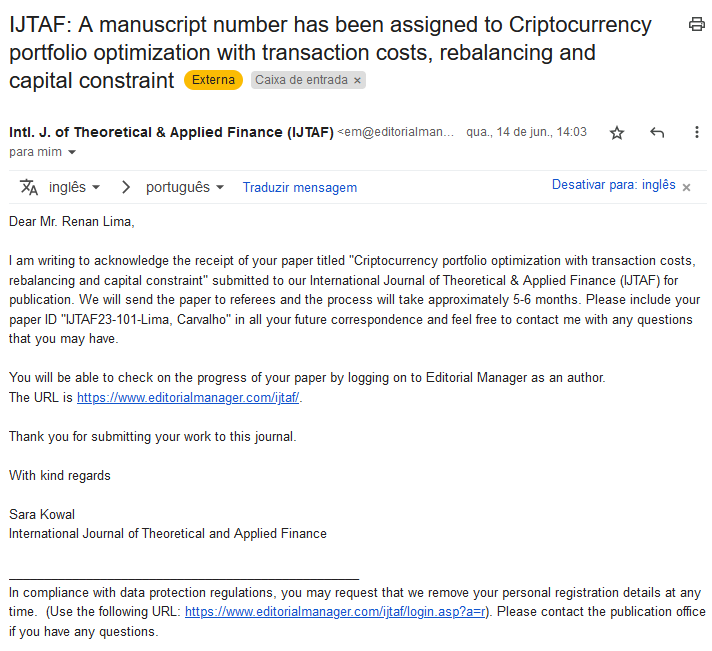
\includegraphics[width=.9\textwidth]{./imagens/ijtaf.png}
                \end{figure}

            \pagebreak
            
            \item LV Simpósio Brasileiro de Pesquisa Operacional
            
                \begin{figure}[htbp]
                    \centering
                    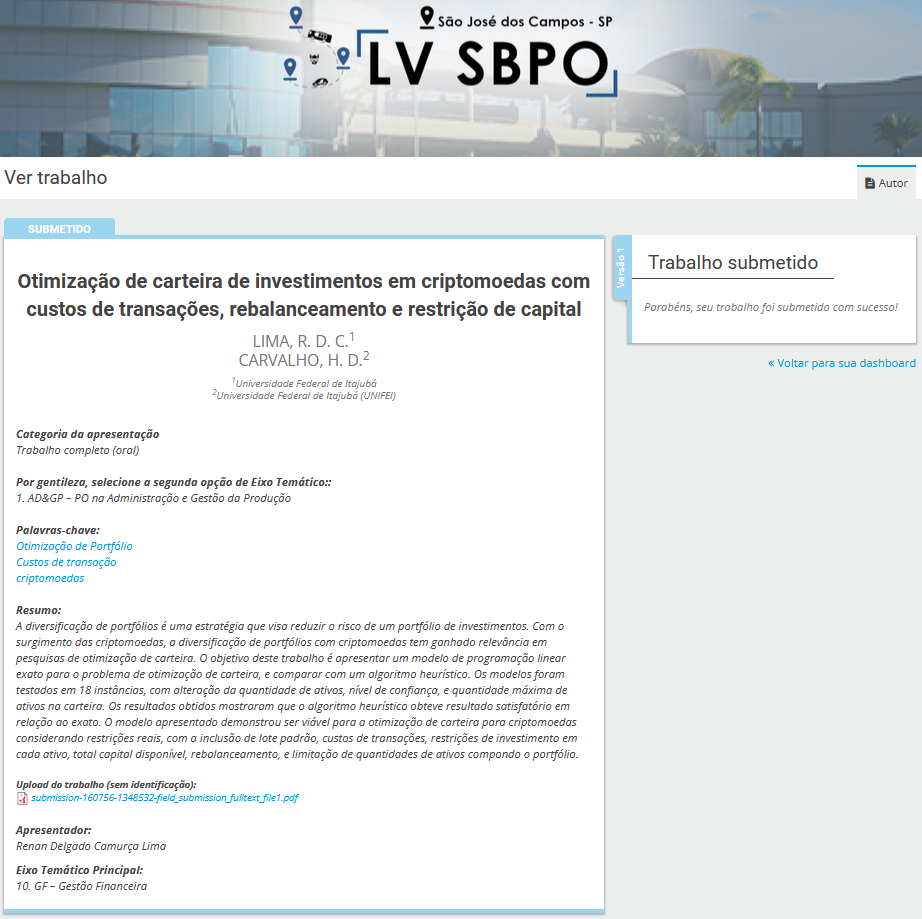
\includegraphics[width=.9\textwidth]{./imagens/sbpo.png}
                \end{figure}

            
        \end{enumerate}

\pagebreak